\chapter{Transferring it to the Real World}
\label{sec:tradeoff}


After having created a set of 2D images, the final step applies low-level image transformations. It allows to further simulate sensor effects and increase the variance in the generated data.

In literature \cite{Krizhevsky2012a,Howard2013,Redmon,Liu} the application of image augmentation is a common tool to improve the detection performance. The experiments in \cite{Carlson2018} show how the incorporation of sensor effects particularly improves the performance of models learned on fully synthesized data. In the \ac{MAV} domain sensor and lens effects have a significant influence on the obtained sample. Hence, we hypothesize that the incorporation of these effects is particularly useful for the \ac{MAV} domain.

\paragraph{Lens Distortion}

Lens distortion is a form of optical aberration which causes light to not fall in a single point but a region of space. For \acp{MAV} commonly used wide-angle lenses, this leads to barrel distortion and thus to straight lines appearing as curves in the image.

The effect is applied using the model for wide-angle lenses from \cite{Vass}. It models the removal of lens distortion as combination of radial and non-radial part, that is approximated with a second order Taylor expansion:
\todo{double check formula is (y in first line?)}
\begin{equation}
f(x,y) =
\begin{pmatrix}
x (1 + \kappa_1 x^2 + \kappa_1 (1 + \lambda_x) y^2 + \kappa_2(x^2 + y^2)^2) \\
y (1 + \kappa_1 x^2 + \kappa_1 (1 + \lambda_y) y^2 + \kappa_2(x^2 + y^2)^2)
\end{pmatrix} 
\label{eq:distortion}
\end{equation}
Where:
\begin{itemize}
	\item f yields the undistorted coordinates.
	\item $\kappa_1$ $\kappa_2$ control the radial distortion 
	\item $\lambda_x$ and $\lambda_y$ control the tangential distortion
\end{itemize}

Applying the lens distortion to an image is done using the inverse of \Cref{eq:distortion}. However, as there is no closed form solution, so the Newton-approximation.

An example with $\kappa_1 = 0.5, \kappa_2 = 0.5$ is displayed in \Cref{fig:distortion}. It can be seen how the previously straight lines appear as circular shape.

\paragraph{Chromatic Aberration.}

Chromatic Aberration is caused when different wavelengths of light do not end up in the same locations of the visual sensor. This leads to a shift in the colour channels of the image.

Similarly to \cite{Carlson2018}, chromatic aberration is applied by scaling the locations of the green channel, as well as applying translations on all channels. The model can be implemented as affine transformation of the pixel locations for each channel:

\begin{equation}
f(x_C,y_C) = \begin{pmatrix}
S & 0 & t_x \\
0 & S & t_y \\
0 & 0 & 1
\end{pmatrix} \begin{pmatrix}
x_C \\
y_C \\
1
\end{pmatrix}
\end{equation}

Where $C$ is one colour channel of the image.

An example is displayed in \Cref{fig:chromatic}. It can be seen how the red and green channel are shifted relative to each other. Thus two bars appear in the image.

\paragraph{Blur}

Motion noise is caused when light falls in different locations of the images sensor due to a fast movement of the camera. It leads to blurry images based on the sensor motion.

The phenomenon depends on camera properties as well as the motion of camera and objects. Although a full modelling of this process might benefit the learning process, it requires a complex pipeline and is computationally expensive. Therefore a strong simplification is used, namely a one-dimensional Gaussian filter:

An example for vertical blur is displayed in \Cref{fig:motionblur}. It can be seen how particularly horizontal lines appear softer.

Next to motion, sensor noise can lead to blurry images. For the blur operation a 2D Gaussian kernel is applied on the input image with:

\begin{equation}
k = \frac{1}{2\sigma_x\sigma_y\pi}e^{-\sqrt{\frac{x^2 + y^2}{2\sigma_x\sigma_y}}} 
\end{equation}
\todo{double check notation}
\paragraph{Exposure.}

Exposure is the time the sensor records light in order to create an image. Over- and Underexposure are caused when this time is too short or too long, leading to too dark or too bright images.

Following the model from \cite{Carlson2018}:

\begin{equation}
f(S) = \frac{255}{1 + e^{-A S}}
\end{equation}
where $A$ is a constant term for contrast and $S$ the exposure.
\todo{whats a}
The image can be re-exposed with:

\begin{equation}
I' = f(S+\Delta S)
\end{equation}

where $S$ is obtained from :
\begin{equation}
S = f^{-1}(I)
\end{equation}

An example for overexposure is displayed in \Cref{fig:exposure}. It can be seen how lighter areas appear particularly light, while dark areas remain dark.

\subsection{Color Variations}

\todo{describe hsv scaling}


\begin{figure}[htbp]
	\centering
	\begin{minipage}{0.33\textwidth}
		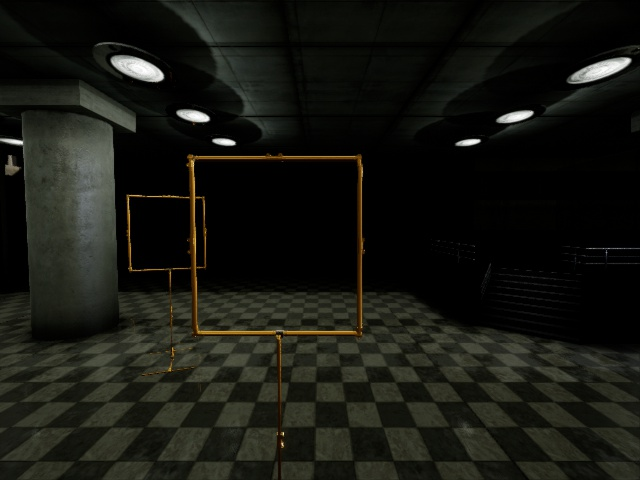
\includegraphics[width=\textwidth]{fig/gate_example}
		\caption{Original Image.}
		\label{fig:orig}
	\end{minipage}
	\begin{minipage}{0.33\textwidth}
		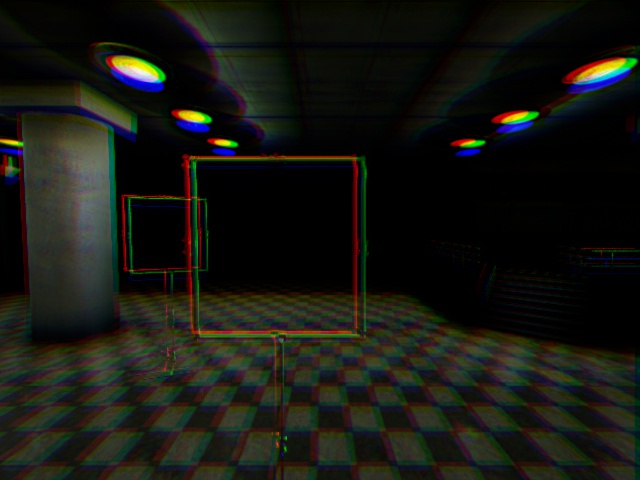
\includegraphics[width=\textwidth]{fig/gate_example_chromatic}
		\caption{Chromatic Aberration.} 		
		\label{fig:chromatic}
	\end{minipage}
	\begin{minipage}{0.33\textwidth}
		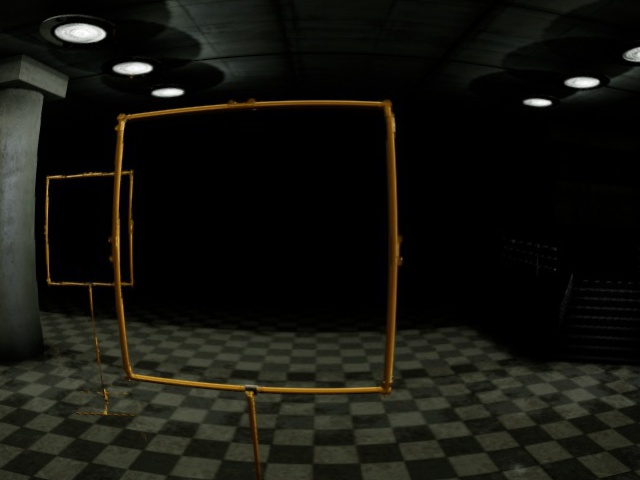
\includegraphics[width=\textwidth]{fig/gate_example_distorted}
		\caption{Lens Distortion. }		
		\label{fig:distortion}
	\end{minipage}
	
	\begin{minipage}{0.33\textwidth}
		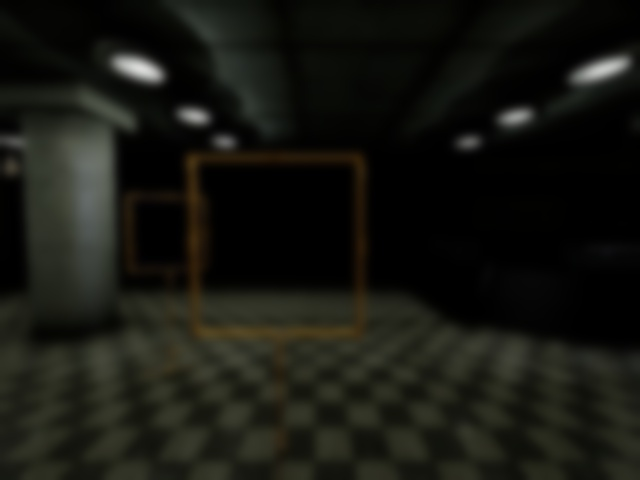
\includegraphics[width=\textwidth]{fig/gate_example_focusblur}
		\caption{Out-of-Focus blur.}
		\label{fig:focusblur}
	\end{minipage}
	\begin{minipage}{0.33\textwidth}
		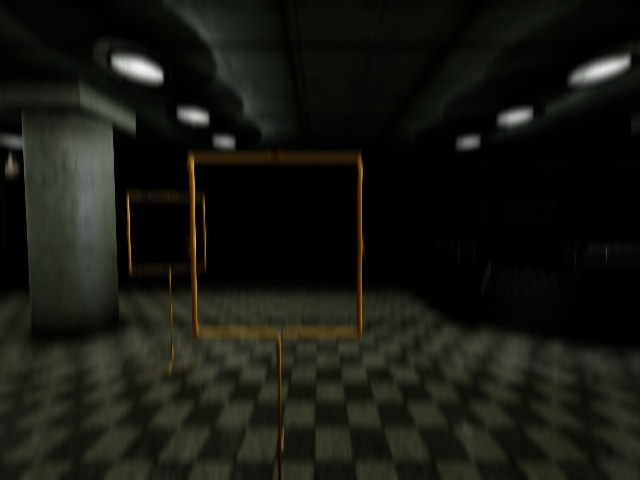
\includegraphics[width=\textwidth]{fig/gate_example_motionblur_v}
		\caption{Vertical Motion Blur.}
		\label{fig:motionblur}
	\end{minipage}
	\begin{minipage}{0.33\textwidth}
		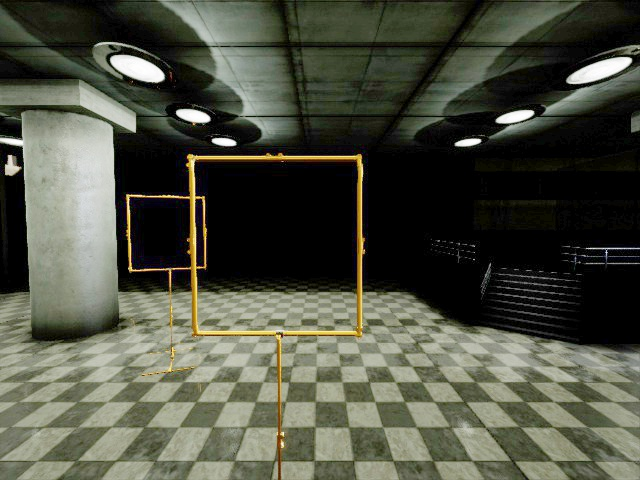
\includegraphics[width=\textwidth]{fig/gate_example_exposure}
		\caption{Exposure.}
		\label{fig:exposure}
	\end{minipage}
\end{figure}

\subsection{Hypothesis}
\label{sec:training:hypothesis}

This chapter summarizes the hypotheses formulated in the previous chapters:

\begin{enumerate}
	\item[$\mathcal{H}_1$] An object that is not empty and provides a more distinctive structure is less background dependent than an \ac{EWFO}.
	
	\item[$\mathcal{H}_2$] The incorporation of correct placement/light conditions improves the performance of a model trained to detect \acp{EWFO}.
	
	\item[$\mathcal{H}_3$] The incorporation of a camera motion model resembling the target domain improves the performance of a model trained to detect \acp{EWFO}. 
	
	\item[$\mathcal{H}_3$] Including sensor effects present in the target domain, improves the performance of a model trained to detect \acp{EWFO}. 
	
\end{enumerate}



\section{Experiments}
\label{sec:training:experiments}
In order to evaluate the formulated hypotheses several experiments are conducted. The model used is the TinyYoloV3-Architecture, further described in \Cref{sec:object_detection}. The reported metrics are described in \Cref{sec:metrics}. For all experiments mean and standard deviation of 5 runs are reported.

For the random view point generation the following parameters are used:

\begin{equation}
x = \mathcal{U}(-30,30),\quad y = \mathcal{U}(-20,20),\quad z = \mathcal{N}(-4.5,0.5)),\quad
\phi = \mathcal{U}(0,0.1\pi),\quad \theta = \mathcal{U}(0,0.1\pi),\quad \psi = \mathcal{N}(-\pi,\pi)
\label{eq:distroexp}
\end{equation}
Where $ \mathcal{U}(a,b)$ is a uniform distribution between $a,b$ and $\mathcal{N}(\mu,\sigma^2)$ is a Gaussian distribution with mean $\mu$ and variance $\sigma^2$.

The parameters are chosen experimentally aiming to resemble common view points of a person standing in the room.

\subsubsection{Experiment I}
The empty space of an \ac{EWFO} is augmented with a detailed texture. An example can be seen in \Cref{fig:cats}.
\begin{figure}
	\centering
	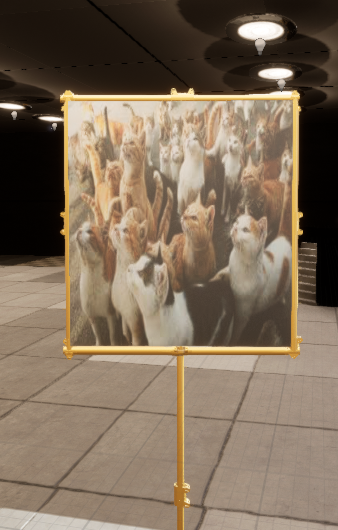
\includegraphics[height=5cm]{fig/cat}
	\caption{The \ac{EWFO} is augmented with a detailed texture.}
	\label{fig:cats}
\end{figure}

The object is placed in a scene with uniformly coloured backgrounds and a training set of 20 000 samples is created. In similar fashion a training set is created without the texture rich augmentation. The test set contains 1000 samples created in the \textit{IROS} environment by randomly placing the camera following \Cref{eq:distroexp}.




\subsubsection{Experiment II}

Several models are trained on 20 000 samples each.
\begin{itemize}
	\item[ModelU] Uniform
	\item[ModelSVE] Single Virtual Environment
	\item[ModelRB] Real Backgrounds
	\item[ModelVVE] Various Virtual Environments
	\item[ModelRBVVE] Real Backgrounds + Various Virtual Environments
\end{itemize}


\begin{table}[htbp]
	\caption{}
	\begin{tabular}{|l|l|l|l|r|r|r|l|l|l|}
		\hline
		& Validation Set &  &  & \multicolumn{1}{l|}{IROS2018} & \multicolumn{1}{l|}{} & \multicolumn{1}{l|}{} & Real Data &  &  \\ \hline
		& AP40 & AP60 & AP80 & \multicolumn{1}{l|}{AP40} & \multicolumn{1}{l|}{AP60} & \multicolumn{1}{l|}{AP80} & AP40 & AP60 & AP80 \\ \hline
		U &  &  &  & 0.05 & 0.01 & 0 &  &  &  \\ \hline
		SVE &  &  &  & 0.29 & 0.17 & 0.02 &  &  &  \\ \hline
		VVE &  &  &  & 0.61 & 0.49 & 0.17 &  &  &  \\ \hline
		RB &  &  &  & 0.42 & 0.28 & 0.04 &  &  &  \\ \hline
	\end{tabular}
	\label{tab:env}
\end{table}


\subsubsection{Experiment III}

Three models are trained: Model I using random placement, Model II using the drone motion model, Model III using a combination of both methods. In both experiments environment and light conditions as well as object locations are the same. The models are tested on two test sets: Set I created by randomly placing the camera. Set II by using the drone motion model, where a circuit is used that has not been part in the generation of the training data.


\subsubsection{Experiment IV}

In order to evaluate $\mathcal{H}_4$ the individual domain properties are measured on the target domain and incorporated in the training set.


\section{Results}
\label{sec:training:results}

\section{Discussion}
\label{sec:training:discussion}

\section{Conclusion}
\label{sec:training:conclusion}


